\pagebreak

\section{Zynq ARM processor interface Library - xilinx/zynq\_axi.3pl}
\label{chap:lmzynqaxilib}

    \index{library!xilinx/zynq\_axi.3pl}
    This library instantiates a Zynq CPU and provides interfaces to
    the two general purpose memory-mapped slave buses and the four
    high performance DMA master buses. It also connects the DDR RAM
    and general purpose I/O pins to the CPU.
    
    This library must be incorporated by using a {\bf source} statement -
    \begin{lstlisting}[gobble=4, language=threepl]
       source "xilinx/zynq\_axi.3pl"
    \end{lstlisting}

    however xilinx/zynq\_axi.3pl is already included in board header files -\\
    boards/avnet/microzed\_7010.3pl\\
    boards/avnet/microzed\_7020.3pl\\
    boards/digilent/zybo.3pl
    
    Code to create the interface to the CPU must be executed as a trailer module
    by -
    
    \begin{lstlisting}[gobble=4, language=threepl]
        trailermodule ("zynq processor") {
            zynq_ps();
        }
    \end{lstlisting}
    and this is also incorporated in the header files listed above.

    Application code only needs to incorporate the board header file
    and create an instance of the CPU interface, e.g. -

    \begin{lstlisting}[gobble=4, language=threepl]
        module "boards/avnet/microzed_7010.3pl"

        class(cpu, cpu_api());
    \end{lstlisting}
    The CPU\_API class is documented in
    \autorefph{chap:lmxilcpulib} {\bf FPGA to CPU interface Library
    - xilinx/cpu.3pl}. This library can also be used by FPGA boards
    which have a USB serial interface to a host computer.
   
    Since cpu.3pl is included via a source statement its code shares the scope
    of this library, UART\_CPU. Thus it can call the modules, functions and
    procedures therin.
    
    {\bf cpu.3pl} defines a class {\bf CPU\_API()} which provides the following
    class procedures for data transfer between FPGA and CPU - \\
        \hspace*{1cm}{\bf read()} generic read \autorefph{sec:lpcpurd} \\
        \hspace*{1cm}{\bf write()} generic write \autorefph{sec:lpcpuwr} \\
        \hspace*{1cm}{\bf read\_memory()} memory read \autorefph{sec:lpcpurdmem} \\
        \hspace*{1cm}{\bf read\_queue()} queue read \autorefph{sec:lpcpurdqueue} \\
        \hspace*{1cm}{\bf read\_value()} value read \autorefph{sec:lpcpurdvalue} \\
        \hspace*{1cm}{\bf write\_memory()} memory write \autorefph{sec:lpcpuwrmem} \\
        \hspace*{1cm}{\bf write\_queue()} queue write \autorefph{sec:lpcpuwrqueue} \\
        \hspace*{1cm}{\bf write\_static()} static write \autorefph{sec:lpcpuwrstat} \\
        \hspace*{1cm}{\bf dma\_read()} to FPGA from CPU \autorefph{sec:lpcpudmar} \\
        \hspace*{1cm}{\bf dma\_write()} from FPGA to CPU \autorefph{sec:lpcpudmaw} \\
        \hspace*{1cm}{\bf signal\_interrupt()} interrupt from a signal \autorefph{sec:lpcpusigint} \\
        \hspace*{1cm}{\bf interrupt()} interrupt procedure \autorefph{sec:lpcpuint} \\

    each of which can generate an instance of a CPU interface to a specific 3PL
    variable of appropriate mode. An internal class {\bf CPU\_CODEGEN} is also
    created but this is not visible to the application code 
    
    cpu.3pl is sourced by both {\bf uart\_cpu.3pl} and {\bf zynq\_axi.3pl} to
    provide CPU interfaces. The former employs a serial data link and the
    latter parallel busses.
    
    When any of the procedures above are called a defining structure is
    created which is added to a list of CPU interfaces. At the end
    of immediate execution module {\bf create\_bus\_interfaces()} is called.
    {\bf create\_bus\_interfaces()} is defined in both {\bf uart\_cpu.3pl}
    and {\bf zynq\_axi.3pl} as it is specific to each. This module
    traverses the interface list constructed above and for each interface
    calls a matching procedure in class {\bf CPU\_CODEGEN} to generate the
    logic for each instance.


    
    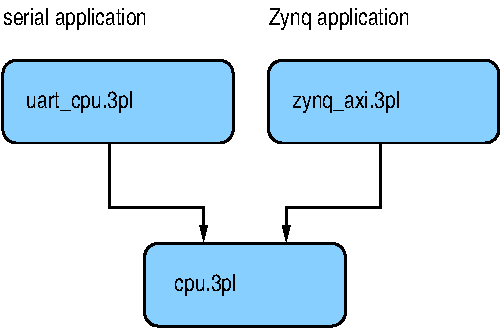
\includegraphics{cpu}
    
    Bus GP0 is used for reading 3PL expression values and queue mode variables
    and writing static and queue mode variables.

    Bus GP1 is used to read and write 3PL memory mode variables.

    For both GP buses burst transfers are used and burst lengths may be up to 8
    32-bit words. Burst transfers are executed in the CPU interface code by
    load/store multiple commands which use a contiguous set of registers. A
    maximum of 8 of the 16 available registers has been imposed, hence the
    maximum burst size of 8 32-bit words.

    An information file, design.info, is generated. This file lists the
    directives, AXI bus interface details and interrupt event parameters. The
    file is in JSON format. A python utility program, info2c,  extracts data
    from this information file and generates a .h file for CPU programs in C.
    Similar utilities may be written for other languages.

    info2c is a shell script invoking python. The first or only argument is the
    design name and info2c expects to find a file design.info. It will create a
    file design.h. If the optional second argument is provided then it is used
    as the output file name (".h" is appended).
    
    The design.info data may also be stored in block RAM (rmemory) for read-time
    access by CPU code. This is enabled by default but may be avoided via a
    directive, i.e. {\bf directive("excludeinfo", true);}, which can be executed
    at any time during 3PL immediate execution. The compression is done by
    calling inbuilt function {\bf deflate()} \autorefph{sec:ifdeflate}. The
    readback is initialised by writing to address 1 and 32-bit packed .info data
    is then read by successive 32-bit reads from address 1. The first read
    returns a 32 bit CRC-32 checksum for the remainder of the block,\. The
    second read returns the uncompressed data size in bytes and the third read
    returns the compressed data size in bytes. Reads beyond the data length will
    return zeros.
    
    The data block size depends on the size of the compressed .info data and
    varies from a minimum of 1024 32 bit words (1 RAM block) to 32,768 words (32
    RAM blocks).

    These bus interfaces allocate successive addresses. These addresses are
    embedded in C functions generated by info2c and hence the programmer does
    not need to know the addresses (they can be determined from the .info file).
    Each interface is supplied a unique name in the 3PL procedure call and this
    name is used in the associated generated function names.

    For 3PL int types info2c will generate matching C types int8\_t, int16\_t,
    int32\_t or int64\_t as appropriate to the size of the datum. The maximum
    primitive size is 64 bits.

    For 3PL uint or bits types info2c will generate matching C types uint8\_t,
    uint16\_t, uint32\_t or uint64\_t as appropriate to the size of the datum.
    The maximum primitive size is 64 bits.

    For 3PL log type info2c will generate matching type bool\_t

    For  3PL structs or enums info2c will generate a matching C bit field
    struct. The maximum size for a struct is 64 bits.

    For a 3PL float type info2c will generate a C float or double type if the
    the type matches IEEE 754 format, otherwise it will generate a C bit field
    struct containing the exponent and mantissa as fields.

    The 3PL data type may be an array of uint, bits or int of exactly 32 or 64
    bits where the dimension is a maximum of 8 for 32 bit members or 4 for 64
    bit members. The matching C type generated will be a struct containing the
    array.



    \subsection{library modules}


        \subsubsection{cpu\_write\_dma\_buffer - DMA transfer to CPU RAM}\label{sec:lmzynqdmabufr}

            {\bf Library: xilinx/zynq\_axi.3pl}

            {\bf Prototype:} \\
            \vsp
            \begin{lstlisting}[gobble=12, language=threepl]
               global module
               cpu_write_dma_buffer (
                   str(name),          // interface name
                   int(blockwords),    // block length in data words
                   int(nblocks),       // number of blocks
                   queue(in),          // data in
                   log(use_wcount),    // use queue count rather than interrupt
                   log(bigendian)      // transfer data as bigendian
               ) {}
            \end{lstlisting}

            {\bf Output parameters:} \\
            none

            {\bf Input parameters:} \\            
            {\bf name} is a string identifier for the interface.\\
            {\bf blockwords} is the DMA block length in data words.\\
            {\bf nblocks} is the number of DMA blocks used.\\
            {\bf in} is a queue of data to be transferred.\\
            {\bf use\_wcount} determines whether an interrupt or a count are
            to be used to determine when to read the 'done' queue.
            
            This module creates a DMA buffer management interface allowing the FPGA
            to write directly to CPU RAM using DMA. For a simpler interface see {\bf
            dma\_write()} \autorefph{sec:lmzynqwrdma}. The parameter {\bf name} is
            used when creating the interface functions for this module.
            
            The interface will use the next unused HP bus of the four available.
            If all four HP buses have been used then a fatal error is invoked.
            
            The interface has two queues accessible to the CPU, a 'free' queue and
            a 'done' queue.
            
            The 'free' queue contains block numbers that are available to the DMA
            for writing. This queue is loaded initially by the CPU. The DMA
            interface removes a block number from the 'free' queue when it is to
            begin writing a block. If this queue is empy then DMA will wait until
            a block number is written to it by the CPU.

            When the DMA has finished filling a block in CPU RAM then it writes
            the block number to a 'done' queue. The block numbers read from the
            'done' queue can be used to compute the associated buffer address in
            mapped DMA memory.
            
            If {\bf use\_wcount} has no argument or the argument value is FALSE
            then there is an interrupt associated with that queue on which the
            CPU can wait for completed blocks to be signalled. The interrupt is
            a level which can be used to control a loop reading one item from
            the queue on each iteration.
            
            If {\bf use\_wcount} has a TRUE argument then the number of block
            numbers queued in the done queue can be determined and read in
            a count-controlled loop.
            
            The CPU must return a block number read from the 'done' queue to the
            'free' queue after it has completed processing the data in the block.
            
            The status of block numbers in the range of blocks available for use
            is recorded in memory in this DMA interface. This status can be used
            when recovering from a CPU crash but not reloading the FPGA
            configuration. The status for a block can be read or written by the
            CPU and will be one of -

            \blist
            \item   missing - the block number is missing from the DMA interface.
            It presumably has been removed by the CPU and not yet returned.
            \item   free - the block is free for a DMA transfer
            \item   done - a DMA transfer has been completed for this block
            \item   busy - the block is currently being written by a DMA transfer
            \blend
                        
            The data input queue {\bf in} must be of type -

            \begin{lstlisting}[gobble=12, language=threepl]
               struct(...,
                   data,       ...user data type ...,
                   term,       dma_block_term,
                   tag,        tagtype
               );
            \end{lstlisting}

            where\\
            \blist
            \item {\bf data} is the user data which can be any type\\
            \item {\bf term} is a block termination enumerated type
            'dma\_block\_term' which is\\
                \blist
                \item {\bf 'none'} (default) to add the datum to the current block\\
                \item {\bf 'ignore'} to terminate the block, discarding the
                accompanying datum\\
                \item {\bf 'first'} to start a new block with the datum
                \item {\bf 'last'} to add the current datum to the block then
                terminate the block\\
                \blend
            \item {\bf tag} is a user-defined field which can be used to
            distinguish blocks of different content. The tag field of the last
            datum to be added to the current block is used as the block tag, all
            previous ones being ignored.
            \blend
            
            The block termination mechanism will not terminate an empty block.

            Blocks will be terminated when full if not explicitly terminated by use
            of the termination field.

            The input data type is rounded up in size to 8, 16, 32 or 64 bits,
            zero padded at the MSB end where necessary.
            Data are packed into 64-bit words for transmission across an HP bus
            to CPU memory. The packing is 8x8, 4x16, 2x32 or 1x64.
            Where a block is terminated before being filled any unfilled portion of
            the last 64-bit word will be zero. The remainder of the block in CPU
            memory remains unwritten.

            On completion of a block transfer the structure that is read by
            the CPU from the 'done' queue is -

            \begin{lstlisting}[gobble=12, language=threepl]
               struct(bnctype,
                  blocknum,    "uint:"+size(nblocks),
                  words,       "uint:"+size(blockwords),
                  tag,         tagtype
               );
            \end{lstlisting}

            where -
            \blist
            \item {\bf blocknum} is the block number in the DMA buffer space\\
            \item {\bf words} gives the number of words of packed user data in the block\\
            \item {\bf tag} is a user-defined block tag\\
            \blend
            
            The Zynq ARM processor is little-endian and this is the default transfer
            order. If the argument to parameter {\bf bigendian} is supplied and is
            true the data will be transferred in big-endian order instead. This
            might be used if the data is to be transferred unprocessed out of the
            Zynq to another processor which is big-endian.



            
            
            The following C functions will be created from the .info file and placed
            into an include file by executing the python script info2c -
            
            \begin{tabular}{| l | l | l |}
            \hline
            fpga\_{\em name}\_done\_read()                  &   & read done queue block number and word count\\ \hline
            fpga\_{\em name}\_done\_avail\_read()           & 1 & read number of words in done queue     \\ \hline
            fpga\_{\em name}\_done\_avail\_thresh\_write()  &   & set interrupt threshold for done queue \\ \hline
            fpga\_{\em name}\_done\_enable()                & 2 & enable done queue interrupt            \\ \hline
            fpga\_{\em name}\_done\_disable()               & 2 & disable done queue interrupt           \\ \hline 
            fpga\_{\em name}\_done\_wait()                  & 2 & wait on done queue interrupt           \\ \hline  
            fpga\_{\em name}\_free\_write()                 &   & write to free queue                    \\ \hline  
            fpga\_{\em name}\_status\_read()                &   & read block status memory              \\ \hline  
            \end{tabular}
            
            Notes:\\
            1 - only if argument wcount is true\\
            2 - only if argument wcount is omitted or false
            
            in addition entries similar to the following will also be placed
            in the include file -
            
            \begin{tabular}{| l |}
            \hline
            const unsigned fpga\_{\em name}\_blocks 4; \\
            const unsigned fpga\_{\em name}\_block\_size 160; \\
            const unsigned fpga\_{\em name}\_block\_words 80; \\
            const unsigned fpga\_{\em name}\_port 0; \\
            typedef uint32\_t fpga\_{\em name}\_t; \\
            \hline
            \end{tabular}

            In the following {\bf fpga} is the pointer to the FPGA
            structure returned by {\bf fpga\_open()}.
            
            {\bf fpga\_{\em name}\_done\_enable(fpga)}
            
            Enable the interrupt on the block completion queue non-empty. This is
            only available if {\bf use\_wcount} is FALSE.
            
            {\bf fpga\_{\em name}\_done\_wait(fpga, NULL)}
            
            Wait on the interrupt on the block completion queue. Execution will
            continue, and the interrupt is disabled, when the queue is not empty.
            This is only available if {\bf use\_wcount} is FALSE. The second
            argument if not NULL is a timeout period (struct timeval).
            
            {\bf fpga\_{\em name}\_done\_avail\_read(fpga)}
            
            Read the availability count on the block completion queue. This is
            only available if {\bf use\_wcount} is TRUE.
            
            {\bf fpga\_{\em name}\_done\_read(fpga)}
            
            Read the block completion queue. The function returns a structure
            similar to the following -
            
            \begin{lstlisting}[gobble=12, language=C]
               typedef union {
                   struct {
                       uint16_t blocknum: 3;
                       uint16_t words: 6;
                       uint16_t blocktype: 2;
                       uint16_t : 5;
                   };
                   uint16_t __word;
               } fpga_{\em name}_done_t;
            \end{lstlisting}
            where {\bf blocknum} is the
            block number of a completed block in the DMA buffer,
            {\bf words} is the number of words of type {\bf fpga\_{\em name}\_t}
            written to that buffer (i.e. data words, not necessarily 64-bit words)
            and {\bf blocktype} is the user's arbitrary block type code. The
            last unnamed field (5) is padding to make up 16 bits.
            
            {\bf fpga\_{\em name}\_free\_write(fpga, blocknum)}
            
            Write a block number to the free block queue for re-use by the
            DMA interface ({\bf blocknum} is just an integer, not the struct
            shown above).

            {\bf fpga\_{\em name}\_status\_read(fpga, blocknum)}
            
            Read the status of a block from the DMA interface.
            For an interface named "xyz" the returned status would be a
            byte of type -
            
            \begin{lstlisting}[gobble=12, language=C]
                typedef enum {
                    fpga_xyz_status_busy = 2,
                    fpga_xyz_status_done = 3,
                    fpga_xyz_status_free = 1,
                    fpga_xyz_status_missing = 0,
                } fpga_xyz_status_t;
            \end{lstlisting}
            
            Any block number that has status 'missing' can be written to the free
            queue to make it once again available for use.
            
            {\bf const unsigned fpga\_{\em name}\_blocks}
            
            The number of DMA blocks for this interface.
            
            {\bf const unsigned fpga\_{\em name}\_block\_size}
            
            The block length in bytes for this interface, rounded up to a
            multiple of 8.
            
            {\bf const unsigned fpga\_{\em name}\_block\_words}
            
            The number of data words in this block.

            {\bf const unsigned fpga\_{\em name}\_port}
            
            The HP bus used for this interface, 0 to 3.
            
            {\bf typedef uint32\_t fpga\_{\em name}\_t}
            
            The type of data word.
            
            The CPU C code (using interrupt) might appear as follows,
            "DMA1" being the interface name -
            
            \begin{lstlisting}[gobble=12, language=C]
                   fpga_t *        fpga = NULL;
                   fpga_DMA_done_t bn;

                   nrete( fpga = fpga_open(fpga_unit_default, fpga_flag_default) );
                   erete( fpga_configdata_load(fpga, prog_fpga_config_data, prog_fpga_config_size) );
                   erete( fpga_map (fpga) );
    
                   // Load the block numbers into the 'free' queue.
                   for (i=0 ; i<HP0_buffers ; i++)
                       fpga_DMA1_free_write(fpga, i);

                   fpga_DMA1_done_enable(fpga);                     // enable interrupt
                   for (;;) {
                       erete( fpga_DMA1_done_wait(fpga, NULL) );
                       // When there is a completed block number available
                       // read it, process the data in the associated buffer,
                       // then return the block number of the now free block.
                       bn = fpga_DMA1_done_read(fpga);             // fetch block number
                       p = fpga->dma.base + bn.blocknum * fpga_DMA1_block_size;
                       for (int i=0 ; i<bn.words ; i++) {
                           .
                           . process data in DMA buffer block pointed to by p
                           .
                       }
                       fpga_DMA1_free_write(fpga, bn.blocknum);    // return block number
                       fpga_DMA1_done_enable(fpga);                // re-enable interrupt
                   }
            \end{lstlisting}

            The code in this module executes in the bus clock domain (c100).
            The clock domain in use when this module is called is restored when
            the module is exited.




        \subsubsection{create\_bus\_interfaces - create the individual CPU interfaces}\label{sec:lmzynqdmabufr}

            {\bf Library: xilinx/zynq\_axi.3pl)}

            {\bf Prototype:} \\
            \vsp
            \begin{lstlisting}[gobble=12, language=threepl]
                module
                create_bus_interfaces () {}
            \end{lstlisting}
            
            {\bf Output parameters:} \\
            
                none.                       
            
            {\bf Input parameters:} \\
            
                none.
                       
            {\bf description:} \\
            This module creates the logic for each of the CPU interfaces. Each
            of these communicates via queues to logic within {\bf zynq\_ps()}
            \autorefph{sec:lpzynqps} below.




    
        \subsubsection{dma\_read - DMA transfer from memory to FPGA}\label{sec:lmzynqrddma}

            {\bf Library: xilinx/zynq\_axi.3pl}


            {\bf Prototype:} \\
            \vsp
            \begin{lstlisting}[gobble=12, language=threepl]
               global module
               dma_read (
                   queue(data, "bits:64")
                   <-
                   int(bus),
                   queue(address, "uint:32"),
                   queue(burstlen, "uint:4")
               ) {}
            \end{lstlisting}

            {\bf Output parameters:} \\Zynq
            {\bf data} is the memory data read

            {\bf Input parameters:} \\            
            {\bf bus} is the high performance master bus, 0 to 3 \\  
            {\bf address} is the physical memory address from which to read \\  
            {\bf burstlen} is the burst length, which is the number of data
            words to be read

            {\bf description:} \\            
            DMA from RAM to FPGA using an AXI HP bus.
            This is a low-level module, providing only a simple DMA interface.
            
            This module can also be called indirectly via library cpu.3pl
            as a procedure in class {\bf CPU\_API}.
            \autorefph{chap:lmxilcpulib} {\bf FPGA to CPU interface Library
            - xilinx/cpu.3pl}.
            
            A datum on each of queues 'address' and 'burstlen' will trigger the
            DMA transfer if queue 'data' is not full. The transfer will consume
            one datum from each of 'address' and 'burstlen' and will write the
            number of data to queue 'data' necessary to satisfy the burst length.
            changed by this procedure,

            The code in this module executes in the bus clock domain (c100).
            The clock domain in use when this module is called is restored when
            the module is exited.



    
        \subsubsection{dma\_write - DMA transfer from FPGA to memory}\label{sec:lmzynqwrdma}

            {\bf Library: xilinx/zynq\_axi.3pl}


            {\bf Prototype:} \\
            \vsp
            \begin{lstlisting}[gobble=12, language=threepl]
               global module
               dma_write (
                   <-
                   int(bus),
                   queue(data, "bits:64")
                   queue(address, "uint:32"),
                   queue(burstlen, "uint:4")
               ) {}
            \end{lstlisting}

            {\bf Output parameters:} \\
            {\bf data} is the memory data read

            {\bf Input parameters:} \\            
            {\bf bus} is the high performance master bus, 0 to 3 \\  
            {\bf address} is the physical memory address to write to \\  
            {\bf burstlen} is the burst length, which is the number of data
            words to be written minus 1

            {\bf description:} \\            
            DMA from PL to RAM using an AXI HP bus.
            This is a low-level module, providing only a simple DMA interface.
            See {\bf cpu\_write\_dma\_buffer()} \autorefph{sec:lmzynqdmabufr}
            for a higher level interface supporting CPU buffer control.
            This is a low-level module, providing only a simple DMA interface.            
            
            This module can also be called indirectly via library cpu.3pl
            as a procedure in class {\bf CPU\_API}.
            \autorefph{chap:lmxilcpulib} {\bf FPGA to CPU interface Library
            - xilinx/cpu.3pl}.
    
            A datum on each of queues 'address' and 'burstlen' will trigger the
            DMA transfer if queue 'data' is not empty. The transfer will consume
            one datum from each of 'address' and 'burstlen' and will read the
            number of data from queue 'data' necessary to satisfy the burst
            length. The 'burstlen' is from 0 for one word to 15 for 16 words.

            The code in this module executes in the bus clock domain (c100).
            The clock domain in use when this module is called is restored when
            the module is exited.

            not empty.

        \subsubsection{sigint - interrupt the CPU on a signal}\label{sec:lmzynqcpusigint}

            {\bf Library: xilinx/zynq\_axi.3pl)}

            {\bf Prototype:} \\
            \vsp
            \begin{lstlisting}[gobble=12, language=threepl]
                module
                sigint(int(n), value(sig, "log")) {}
            \end{lstlisting}
            
            {\bf Output parameters:} \\
            
                none.                       
            
            {\bf Input parameters:} \\
                        
                {\bf n} is the interrupt index, 0 to 16.\\
                {\bf sig} is a signal on whose rising edge the interrupt
                is triggered.\\
                       
            {\bf description:} \\
            When the signal {\bf sig} is asserted the interrupt is triggered.
            The interrupt number, 0 to 15, is given by {\bf index}.



    
        \subsubsection{zynq\_ps - instantiate Zynq CPU}\label{sec:lpzynqps}

            {\bf Library: xilinx/zynq\_axi.3pl}

            {\bf Prototype:} \\
            \vsp
            \begin{lstlisting}[gobble=12, language=threepl]
               module
               zynq_ps () {}
            \end{lstlisting}

            {\bf Output parameters:} \\
            none

            {\bf Input parameters:} \\            
            none
        
            {\bf In-line target execution:} \\
            no

            {\bf description:} \\            
            This instantiates the Zynq CPU and connects the DDR RAM and
            general purpose I/O pins to the CPU. It also defines all the
            CPU pins. After calling this module all the following
            procedures are available.

            The code in this module executes in the bus clock domain (c100).
            The clock domain in use when this module is called is restored when
            the module is exited.



    
    \subsection{library procedures}

                                           
            


        \subsubsection{add\_interface - add an interface to the interface list}\label{sec:lpzynqcpuai}

            {\bf Library: xilinx/zynq\_axi.3pl)}

            {\bf Prototype:} \\
            \vsp
            \begin{lstlisting}[gobble=12, language=threepl]
                procedure
                add_interface (var(v, "->")) {}
            \end{lstlisting}
            
            {\bf Output parameters:} \\
            
                none.
                       
            {\bf Input parameters:} \\
            {\bf v} is an instance of class {\bf busCommon}, defined in
            cpu.3pl.
                     
            {\bf description:} \\
            The instance of {\bf busCommon} is added to the interface list.
            The list is processed at completion of immediate execution to
            create the whole CPU interface.




        \subsubsection{cpu\_read - write to CPU}\label{sec:lpzynqcpurd}

            {\bf Library: xilinx/zynq\_axi.3pl)}

            {\bf Prototype:} \\
            \vsp
            \begin{lstlisting}[gobble=12, language=threepl]
                procedure
                cpu_read (
                    value(access, "log"),
                    value(init, "log"), 
                    queue(out)
                    <-
                    int(bus),
                    int(addr),
                    value(data_in),
                    value(contin, "log")
                ) {}
            \end{lstlisting}
            
            {\bf Output parameters:} \\
            {\bf access} is an optional output parameter which is asserted
            when a CPU to FPGA write occurs.\\
            {\bf init} is an output parameter which is asserted in the case
            of a memory read to initiate the read.\\
            {\bf out} is an optional queue variable which will be written to
            when a transfer occurs.\\

                       
            {\bf Input parameters:} \\
            {\bf bus} is not used (applies to Zynq).\\
            {\bf address} is a 6 bit interface address.\\
            {\bf data\_in} input data.\\
            {\bf contin} is only used for a memory read and is asserted
            when the memory read has occured and the transfer can begin.\\
                     
            {\bf description:} \\
            This procedure provides a low-level interface to transfer
            data from the FPGA to the CPU via the USB serial port. It is
            used by modules and procedures in library cpu.3pl and is not
            intended for use directly by application code.
            
            The CPU initiates the transfer. The transfer may consist of
            multiple bytes.


        \subsubsection{cpu\_write - write to CPU}\label{sec:lpzynqcpuwr}

            {\bf Library: xilinx/zynq\_axi.3pl)}

            {\bf Prototype:} \\
            \vsp
            \begin{lstlisting}[gobble=12, language=threepl]
                procedure
                cpu_write (
                    var(out),
                    value(access, "log")
                    <-
                    int(bus),
                    int(addr)
                ) {}
            \end{lstlisting}
            
            {\bf Output parameters:} \\
            {\bf var} is a static or queue mode variable.\\          
            {\bf access} is an optional output parameter which is asserted
            when a CPU to FPGA write occurs.\\
                       
            {\bf Input parameters:} \\
            {\bf bus} is not used (applies to Zynq).\\
            {\bf address} is a 6 bit interface address.\\           
                     
            {\bf description:} \\
            This procedure provides a low-level interface to transfer
            data from the CPU to the FPGA via the USB serial port. It is
            used by modules and procedures in library cpu.3pl and is not
            intended for use directly by application code.
            
            The CPU initiates the transfer. The transfer may consist of
            multiple bytes.





    \subsection{library functions}
            

        \subsubsection{cpu\_api - CPU communications interface}\label{sec:lfcpuapi}

            {\bf Library: xilinx/zynq\_axi.3pl)}

            {\bf Prototype:} \\
            \vsp
            \begin{lstlisting}[gobble=12, language=threepl]
               global function
               cpu_api () {}
            \end{lstlisting}

            {\bf Return mode and type:} \\
            immediate, class

            {\bf Input parameters:} \\            
            
            none.
            
            {\bf description:} \\
            This function returns an instance of class CPU\_API

            {\bf Library: xilinx/zynq\_axi.3pl}

            {\bf Prototype:} \\
            \vsp
            \begin{lstlisting}[gobble=12, language=threepl]
                global function cpu_api () {}
            \end{lstlisting}
    
        None.




    \subsection{library classes}
    
        None.


